\FloatBarrier
\begin{figure*}[t]
\centering
\begin{subfigure}[b]{0.42\textwidth}
  \centering
  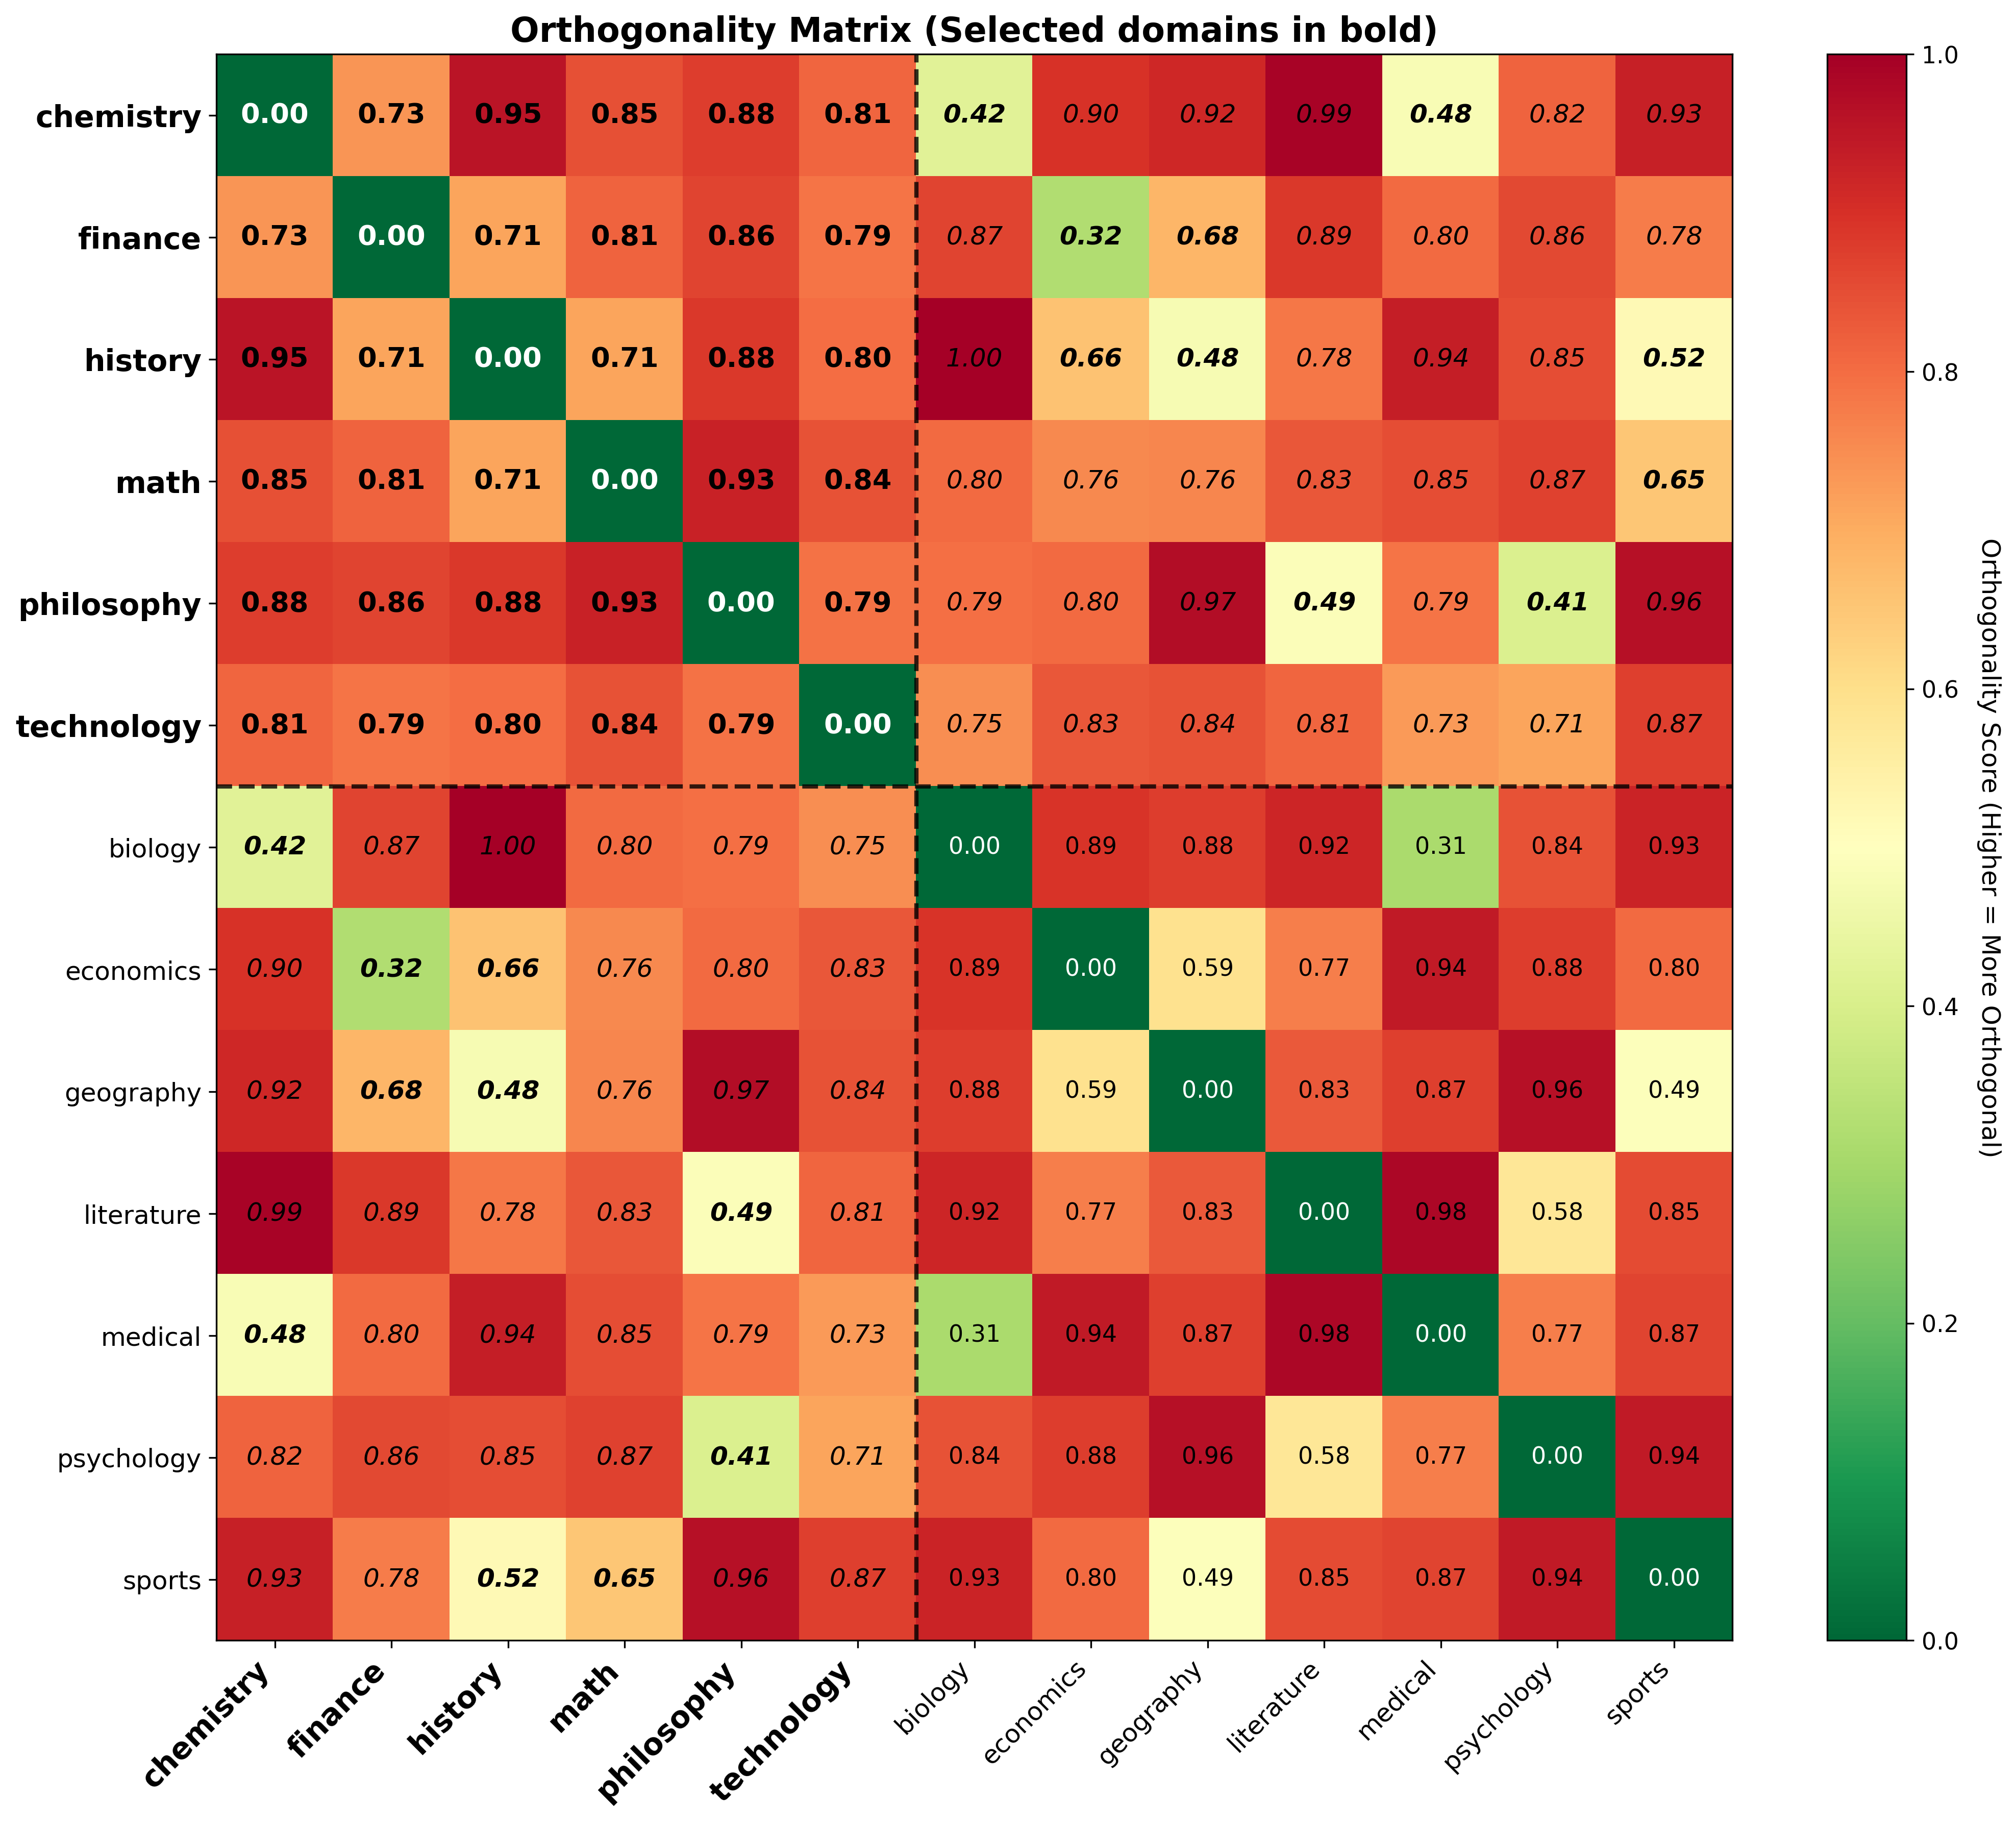
\includegraphics[width=\textwidth]{figs/filtered_orthogonality_matrix.png}
  %\caption{Orthogonality Matrix}
  \label{fig:embed_axes:ortho}
\end{subfigure}
%\hfill
\begin{subfigure}[b]{0.41\textwidth}
  \centering
  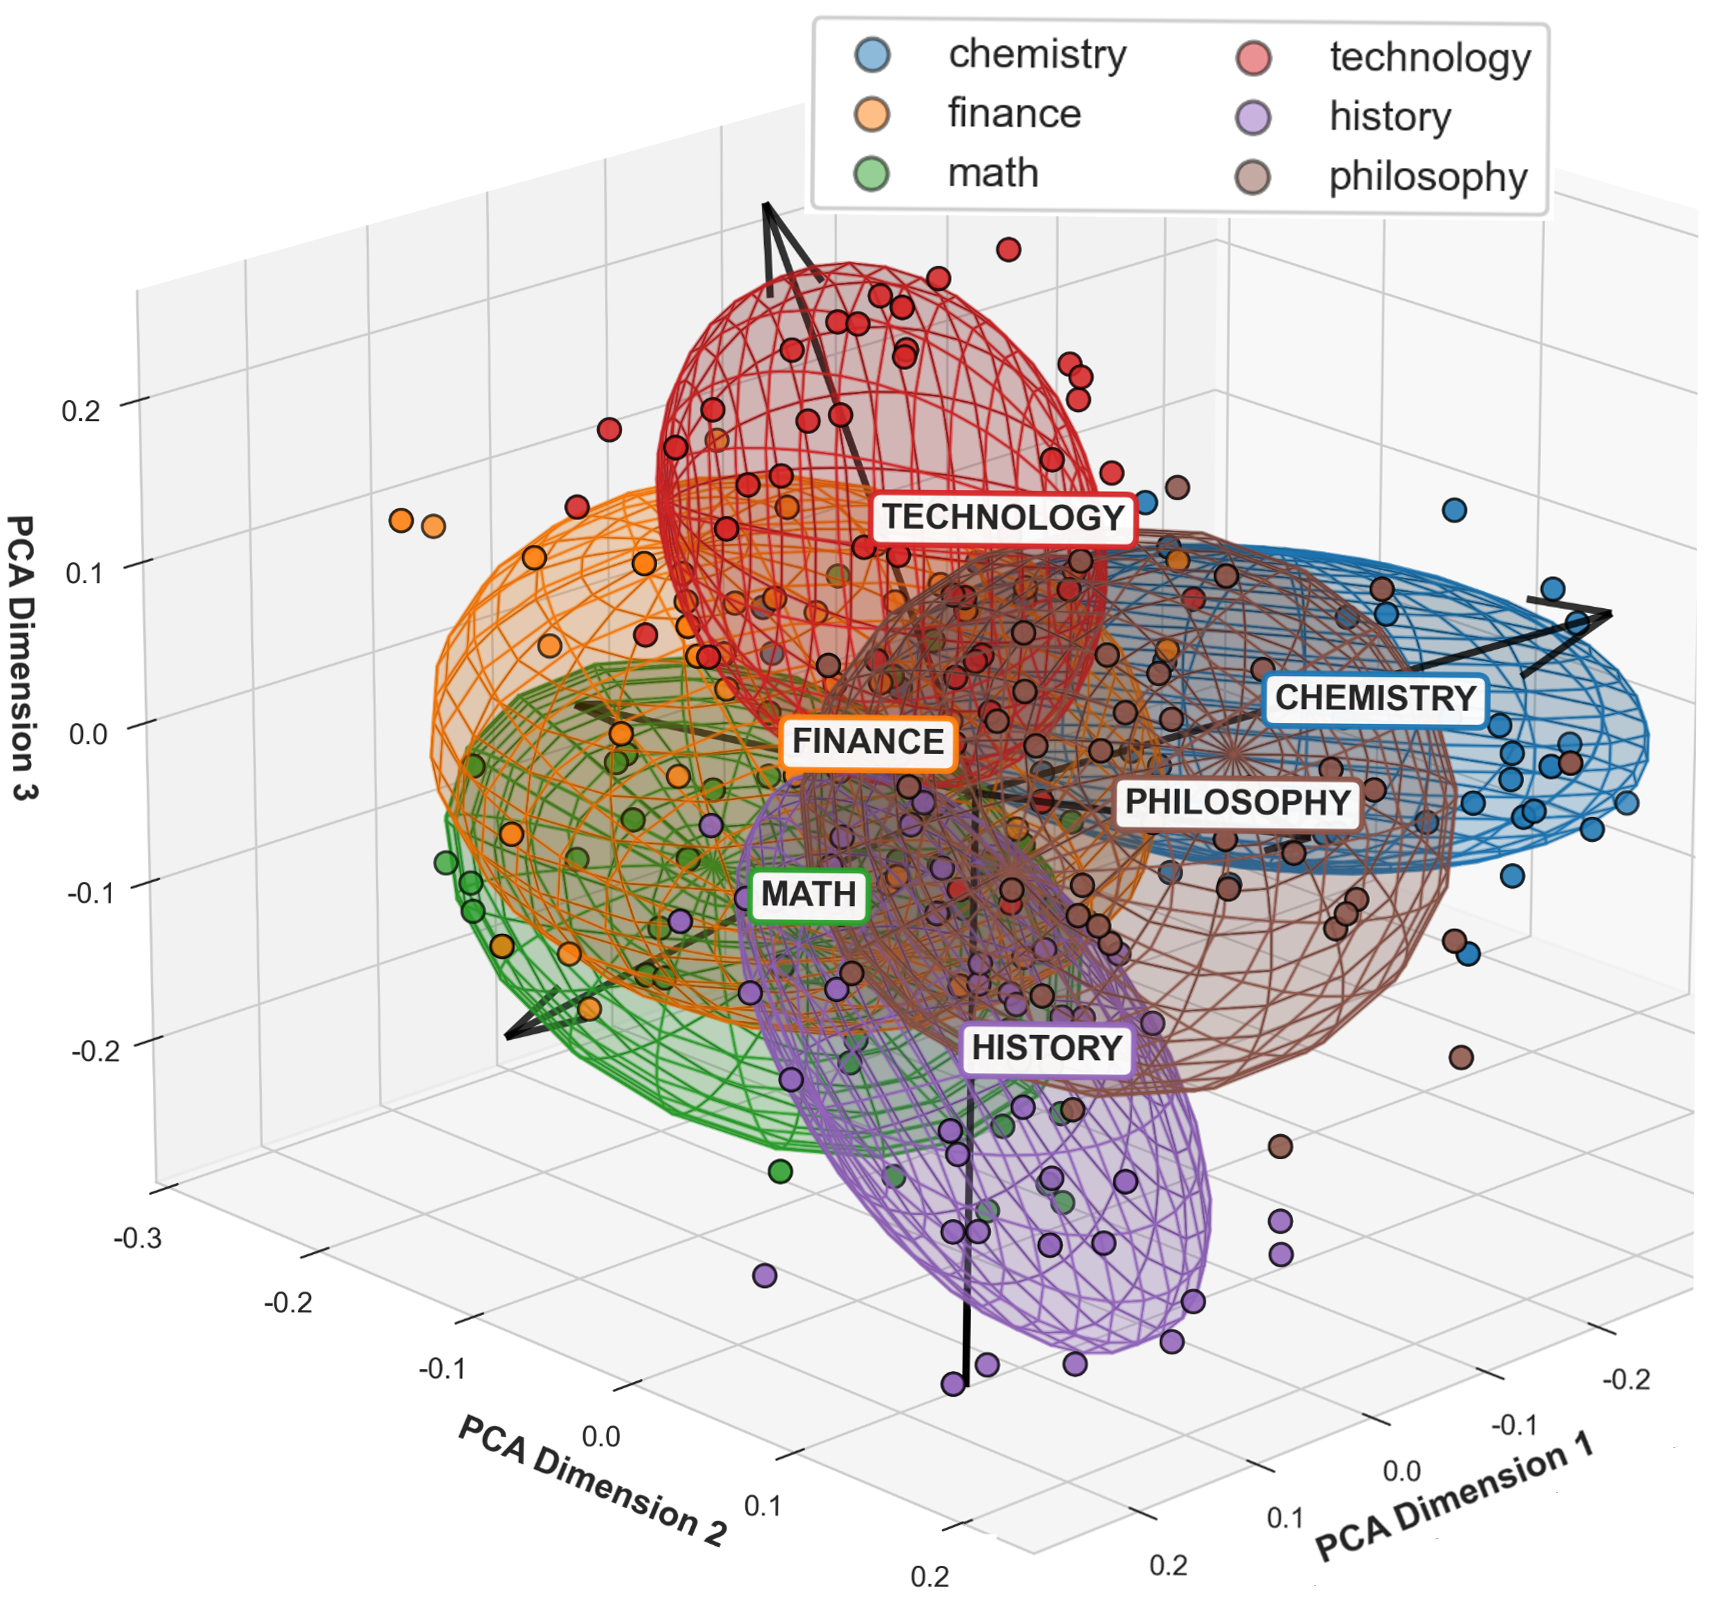
\includegraphics[width=\textwidth]{figs/embedding_space_projection_3d.png}
  %\caption{3D Embedding Projection}
  \label{fig:embed_axes:3d}
\end{subfigure}
\vspace{-6mm}
%\hfill
%\begin{subfigure}[b]{0.32\textwidth}
%  \centering
%  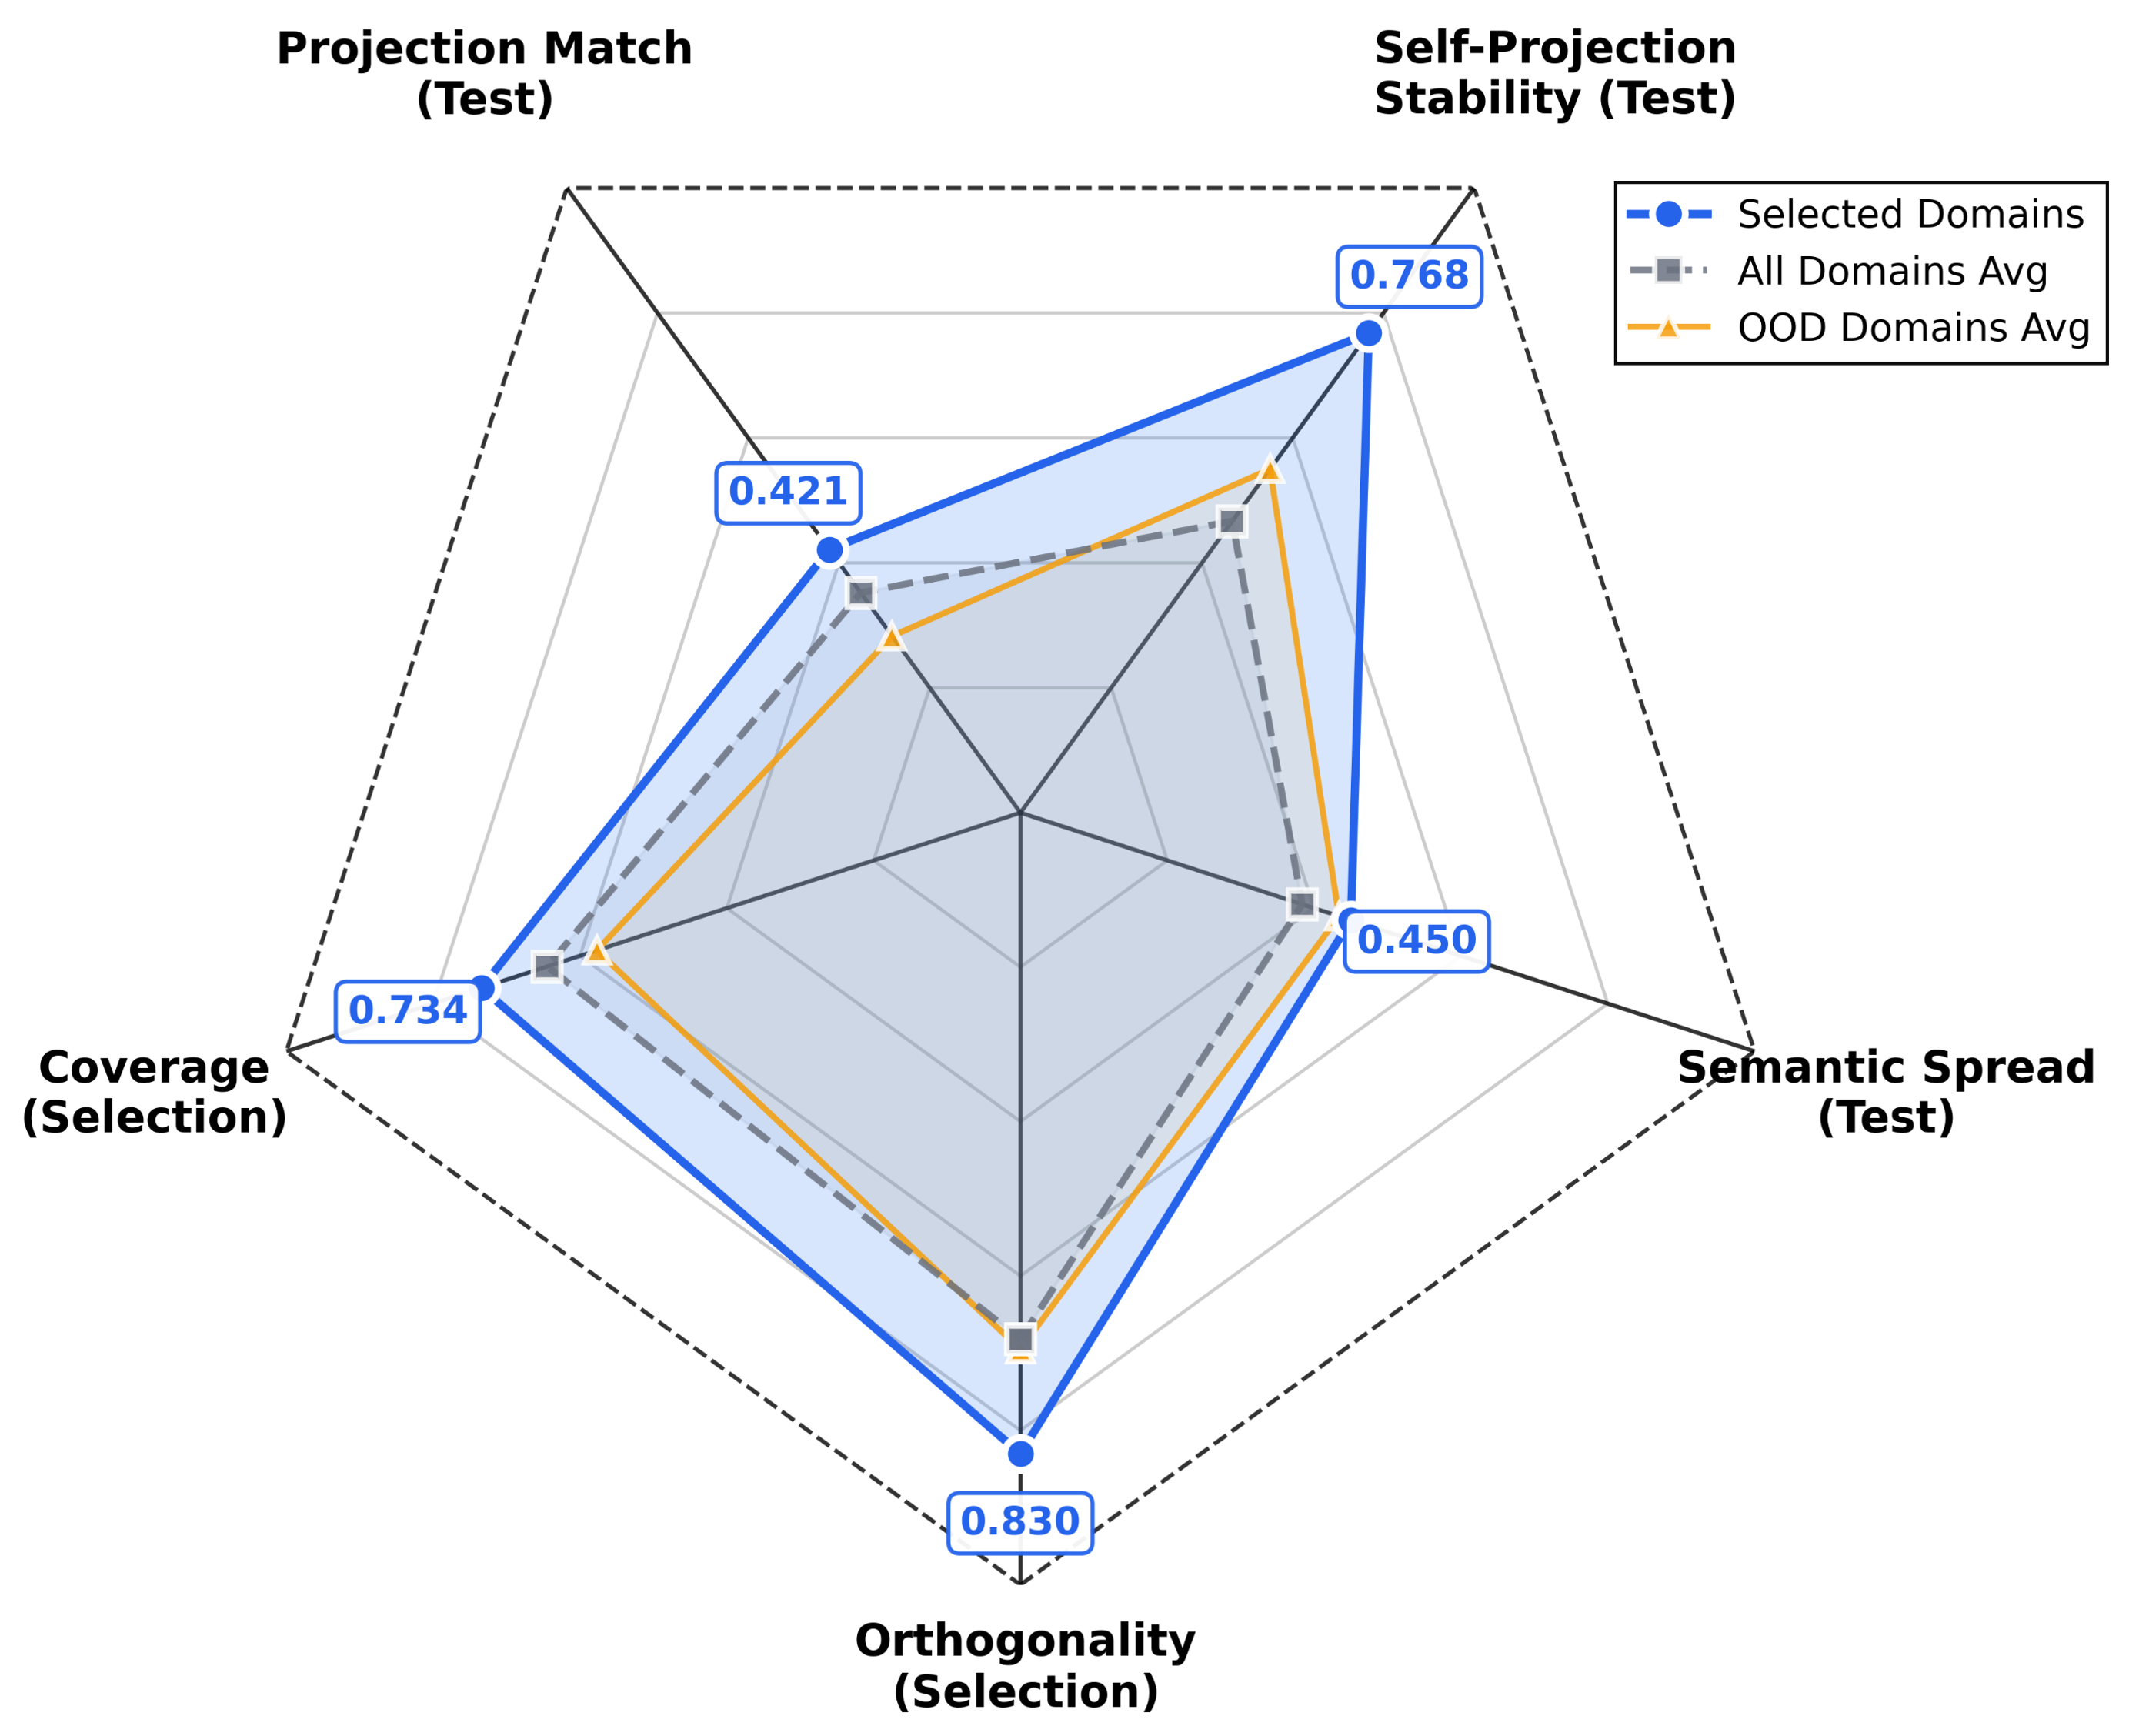
\includegraphics[width=\textwidth]{figs/radar_chart.png}
%  \caption{Metrics Comparison}
%  \label{fig:embed_axes:radar}
%\end{subfigure}
\caption{\textbf{Separation of Domain representation in embedding space.} (Left) Orthogonality heatmap across domains. (Right) Projection of the selected domain showing spatial separation. %(Right) Metrics comparison: Orthogonality and Coverage (selection criteria); Semantic Spread (inter-domain diversity), Self-Projection Stability (intra-group consistency), and Projection Match (OOD alignment) (test criteria). Selected domains outperform baselines across all metrics.
}
\label{fig:embed_axes}
\end{figure*}

\vspace{-0.5mm}
\section{Preliminaries \& Motivations}
\label{sec:prelim}
\vspace{-5pt}

%This section formalizes the objects and assumptions of our \emph{deployment-time training-free} specialization setting and presents \emph{empirical evidence} that motivates our core design.

\subsection{Problem Formulation}
\label{sec:prelim_notation}
\vspace{-5pt}

We consider inference-time settings in which a frozen pre-trained model is repeatedly invoked within a coherent context, denoted as \emph{scenario}. In our pipeline, only inputs~(i.e., queries) are observable, while the ground truth is unavailable to avoid data leaks.

\textbf{Representation subspaces in embedding space.}
We treat embedding space as an ambient $d$-dimensional vector space $\mathbb{R}^d$ in which token-level embeddings live.
Suppose we have access to a small collection of coarse semantic domain sources (e.g., topical repositories or application-specific query banks), which we use solely as an indexing device to construct an embedding-space structure.

Let $\mathcal{K}=\{1,\dots,M\}$ index these domain sources, and $\mathcal{X}$ denote the input space. For each domain $k\in\mathcal{K}$, we are given a input-only pool $\mathcal{P}_k=\{x_i\}_{i=1}^{N_k}\subset\mathcal{X}$. 
Let $\phi:\mathcal{X}\rightarrow\mathbb{R}^d$ be a fixed, non-learned sequence-to-vector map, implemented by mean-pooling frozen backbone token embeddings after stopword filtering, which produces one embedding vector $\mathbf{e}(x)=\phi(x)\in\mathbb{R}^d$ per input and is used only to define the DBS representation coordinate without being trained, routed, or updated during pruning.
We form the embedding set $\mathcal{E}_k \;=\;\{\mathbf{e}(x): x\in \mathcal{P}_k\}\subset\mathbb{R}^d$, 
and build $\mathcal{E}_k$ by a low-dimensional linear \emph{subspace} $\mathcal{U}_k \subset \mathbb{R}^d$ estimated from $\mathcal{E}_k$ via PCA~\cite{abdi2010pca,fernando2013unsupervised,gong2012geodesic,vidal2011subspace}.
Intuitively, $\mathcal{U}_k$ captures dominant embedding-space directions associated with pool $k$; throughout, we call $\mathcal{U}_k$ as \emph{axis} for brevity.
We denote the collection of candidate axes by $\mathbb{U}=\{\mathcal{U}_k\}_{k\in\mathcal{K}}$.

\textbf{Reasoning pathways in parameter space.}
Let $f_\theta$ be a pretrained Transformer with parameters $\theta$ and $h$-head $L$ layers. We index attention heads by $\mathcal{H}=\{(\ell,h): \ell\in\{1,\dots,L\},\, h\in\{1,\dots,H_\ell\}\}$.
\emph{Pathways} are structured computational routes realized by head-wise components across layers. Scenario-specific pruning is represented by a binary sign $m \in \{0,1\}^{|\mathcal{H}|}$, 
indicating which head-wise components are retained~\cite{voita2019heads}.

\textbf{Pruned subnetworks and residual-stream slice.}
A pathway pruning $m$ yields an executable pruned instance as a \emph{subnetwork}. We write $f_{\theta}^{(m)}$ for the model obtained after disabling the head-wise components indicated by $m$.

For an input $x\in\mathcal{X}$, $r^{(\ell)}(x)\in\mathbb{R}^d$ denotes the \emph{post-attention residual stream} at layer $\ell$ averaged across tokens\cite{elhage2021framework} as an observation cross-section to measure the alignment of subspace/axis $\mathbb{U}$.
For $\ell\in\{1,\dots,L\}$ and $k\in\mathcal{K}$, we denote a generic axis-referenced alignment signal by $\alpha^{(\ell)}_k(x)\in\mathbb{R}$, 
whose estimator is specified later.

\subsection{Problem Statement: Inference-time Specialization}
\label{sec:prelim_problem}
\vspace{-0.5mm}
Given a frozen foundation model $f_\theta$ and a specific scenario $s$ with input streams $\{x_t\}_{t=1}^{T_s}$ ($x_t\in\mathcal{X}$), our goal is to compile a budget-bounded pathway pruning $m_s$ once at scenario start and reuse it throughout the scenario, yielding an executable pruned instance $f_{\theta}^{(m_s)}$~\cite{wan2023efficientllm_survey}.

\subsection{Empirical Motivation}
\label{sec:prelim_empirical}
\vspace{-0.5mm}
We provide empirical evidence for \textbf{Subspace--Pathway Coupling}, which serves as the foundational motivation for our framework.
Concretely, (i) domain pools induce a compact and separable distribution in embedding that supports \textbf{DBS},
and (ii) axis-referenced readouts from residual-stream provide a reliable \emph{subspace$\rightarrow$pathway} coupling signal that supports \textbf{PSP}.

\textbf{Evidence 1: Domain pools induce separable distribution.}
Across domain pools $\{\mathcal{P}_k\}_{k\in\mathcal{K}}$, embedding vectors form low-rank subspaces $\{\mathcal{U}_k\}$ that are often well-separated under subspace similarity measures (e.g., principal angles, CKA-style comparisons)~\cite{kornblith2019similarity} shown in Figure~\ref{fig:embed_axes}.
This indicates that embedding space inherently provides a stable coordinate from which a quasi-orthogonal axis basis can be constructed for downstream measurements. We deem this evidence to have the potential to positively affect various router-based approaches.

\textbf{Evidence 2: Subspace-pathway alignment is noteworthy.}
For inputs $x\in\mathcal{X}$, residual-stream slices $r^{(\ell)}(x)$ exhibit consistent correspondence to embedding-level subspaces to some extent, enabling axis-referenced alignment readouts such as $\alpha^{(\ell)}_k(x)$~\cite{alain2016linearprobes,belinkov2022probing,tenney2019bertpipeline,hewitt2019structuralprobe,jawahar2019bertstructure} shown in Figure~\ref{fig:align_pathway}.
Moreover, effective scenario-specific computation is concentrated on a small subset of heads, and the influential subset varies systematically with axis-aligned patterns (e.g., reflected by $\alpha^{(\ell)}_k$), consistent with prior observations of highly non-uniform head contributions~\cite{michel2019sixteen,voita2019heads}.
In addition, we observe a small subset of heads that is consistently activated across domain pools and scenarios, which is denoted as a domain-invariant whitelist $\mathcal{W}\subseteq\mathcal{H}$~\cite{tenney2019bertpipeline,jawahar2019bertstructure,kovaleva2019darksecrets}.

We further provide a detailed theoretical derivation in Appendix~\ref{app:math_foundations}. Together, these results establish a practical \emph{subspace} $\rightarrow$ \emph{pathway} coupling from embedding-space coordinates to parameter-space execution pathways: semantic axes indicate what scenario information should be preserved, while head pathways determine how such information is executed. This coupling turns pruning from generic parameter removal into scenario-conditioned pathway selection, motivating \textsc{SubspacePath Pruner} in the following section.


%\textbf{Evidence 2: Axis-referenced alignment is measurable from residual slices.}
%For inputs $x\in\mathcal{X}$ (without using ground-truth answers), residual-stream slices $r^{(\ell)}(x)$ exhibit consistent correspondence to embedding-level axes/subspaces to some extent, enabling axis-referenced alignment readouts such as $\alpha^{(\ell)}_k(x)$ \cite{alain2016linearprobes,belinkov2022probing,tenney2019bertpipeline,hewitt2019structuralprobe,jawahar2019bertstructure} (Figure~\ref{fig:align_pathway}).
%This supports that we can estimate which embedding axes are most relevant to the scenario inputs and use these readouts to guide scenario-level pathway compilation.

%\textbf{Evidence 3: Pathway usage is concentrated and partially separable.}
%Effective computation concentrates on a relatively small subset of heads, and the influential subset varies with axis-aligned patterns (e.g., reflected by $\alpha^{(\ell)}_k$), consistent with prior observations of highly non-uniform head contributions \cite{michel2019sixteen,voita2019heads} (Figure~\ref{fig:align_pathway}).
%At the same time, pathway sets are only \emph{partially} separable across axes, consistent with superposition effects \cite{elhage2022superposition}, motivating an offline decoupling stage that increases pathway separability before deployment-time selection.
%In addition, we observe a small subset of heads that is consistently activated across pools and scenarios; we denote this domain-invariant backbone whitelist by $\mathcal{W}\subseteq\mathcal{H}$ and treat it as always-retained components under a budget, consistent with layer-wise evidence that lower-level circuits encode more general linguistic/procedural structure \cite{tenney2019bertpipeline,jawahar2019bertstructure,kovaleva2019darksecrets}.


%\textbf{Summary.}
%Embedding-level separability motivates constructing a compact axis/subspace reference (\textbf{DBC}); residual-slice alignment readouts justify scenario-start diagnosis and compilation (\textbf{PSP}); and concentrated yet partially entangled pathway usage---together with a small domain-invariant backbone set---motivates separability-improving decoupling with an always-keep constraint (\textbf{PPD}). 
%The next section operationalizes these insights into a deployment-time training-free methodology.
